\documentclass[12pt,a4paper]{report}
\usepackage[utf8]{inputenc}
\usepackage{amsmath}
\usepackage{amsfonts}
\usepackage{amssymb}
\usepackage{graphicx}
\usepackage{float}

\input defs.tex
\bibliographystyle{alpha}
\graphicspath{ {./figures/} }



\title{Neural Network Based Decoding over Molecular Communication Channels}
\author{Peter Hartig}

\begin{document}
\maketitle

\begin{abstract}

\end{abstract}

\newpage
\tableofcontents
\newpage
\section{Notation}
The following notation conventions are used 
Expectation
Conditional Probability 
Argmax
Vector Indexing

\section{Introduction}
Characterizing and obtaining information about communication channels is a fundamental barrier to communication. While optimal and sub-optimal strategies for overcoming this barrier in many contexts have enabled vast and effective communication infrastructure, this barrier still limits communication in others. Molecular Communication channels pose a particularly difficult context in which to overcome this barrier as channel characteristics are often non-linear and may be dependent on the specific transmitted information.
In communication contexts, such as wireless, "Pilot" symbol-streams are often used to mitigate the difficultly in obtaining channel information by provide real-time information supporting an underlying channel model. The low symbol rate of Molecular Communication channels often makes such strategies impractical. However, the success of this data-driven technique in wireless channels suggest that perhaps an alternative, data-driven method may be viable in the Molecular Communication context. One potential data-driven method for characterizing these channels is a neural network. Neural networks have shown to be an effective tool in data-driven approximating of probability distributions.
\par

The general communication channel is equivalent to a conditional probability $P(x|y)$, in which $x$ is transmitted information and $y$ is received information.  $P(x|y)$ takes into account the (potentially random) channel through which the information $x$ passes, and random noise added prior to receiving $y$. The communication problem entails optimizing a form of $P(x|y)$ over a set of possible, transmitted information $x$. In general, sub-optimal solutions do not require perfect knowledge of the distribution $P(x|y)$ and may be used when $P(x|y)$ is unknown or impractical to obtain. In this work, a neural network is used to estimate $P(x|y)$.

\section{Background}

\subsection{MLSE}
The form of $P(x|y)$ used for detection in this work is
$\underset{x}{\text{argmin}} \; P(y|x) $ . This optimization, known as Maximum Likelihood Sequence Estimation (MLSE), over the set of all possible $x$ is exponentially complex in the cardinaltiy of $x$ . Information about the communication channel can, however, reduce the complexity of this problem. In order to illustrate this reduction, the following example is proposed.
\par
Consider the communication channel over which a causal, linear, and time invariant combination of a set of the transmitted information is received. 

\begin{equation}
y[k] = \sum_{\mathrm{l=1}}^{\mathrm{L}} a[l]x[k-l]
\end{equation}

In this case, $P(y|x)$ can be rewritten as
$\prod P(y_{\mathrm{i}}|x_{\mathrm{i-L+1}}^{\mathrm{i}}) = \sum
log(P(y_{\mathrm{i}}|x_{\mathrm{i-L+1}}^{\mathrm{i}}) )$.
The sequence of received symbols $\mathbf{y}$ can be equivalently represented the by trellis:

TODO IMPORT Trellis picture
in which each time-point k represents a unique set of L transmitted symbols 
$x[k-l]$ $ \forall l \in {1..L}$. Due to the finite number of states that channel can be in at a given time, MLSE can be performed using the Viterbi Algorithm over this trellis. 

Viterbi Algorithm:

    \noindent\rule[10pt]{\textwidth}{0.4pt}
    {\footnotesize
    \begin{tabbing}
        {\bf given} $P(y_{\mathrm{i}}|x_{\mathrm{i-L+1}}^{\mathrm{i}}) \; \forall i \in {1..N}$ . \\*[\smallskipamount]
        Let $\lambda := \lambda^{k-1}$. \\*[\smallskipamount]
        {\bf for $i = 1..N $} \\
         \qquad \= {\bf for each state $s$ at time $i$}\\
        \qquad \qquad \= 1.\ Let $\mathrm{Path}_{s} := \prox_{\lambda g}(x^{k} - \lambda \nabla f(x^{k}))$. \\
        \> 2.\ {\bf break if} $f(z) \leq \hat{f}_{\lambda}(z, x^{k})$. \\
        \> 3.\ Update $\lambda := \beta \lambda$. \\*[\smallskipamount]
        {\bf return} $\underset{s}{\text{argmin}} \; cost[i] $, $x^{k+1}:=z$.
    \end{tabbing}}
    \noindent\rule[10pt]{\textwidth}{0.4pt}


For finite state, causal channels, MLSE reduces to the Viterbi Algorithm. Note that while Viterbi algorithm does have exponential complexity in the length of the channle (i.e. L), complexity is linear in the length of the sequence. 


\subsection{ViterbiNet}
As suggested in the introduction, despite the reduction in complexity offered by the Viterbi Algorithm for MLSE, the individual metrics used each step of the algorithm 
$P(y_{\mathrm{i}}|x_{\mathrm{i-L+1}}^{\mathrm{i}}) $ require knowledge of the channel which may be difficult to obtain. To estimate this distribution using a neural network, Baye's Rule is used. 
\begin{equation}
P(y_{\mathrm{i}}|x_{\mathrm{1 ... L}}) = 
\frac
{P(x_{\mathrm{1 ... L}}|y_{\mathrm{i}})P(y_{\mathrm{i}})}
{P(x_{\mathrm{1 ... L}})}
\end{equation}

These terms can be interpreted as:

\begin{itemize}
\item $P(x_{\mathrm{1 ... L}}|y_{\mathrm{i}})$
: The probability of being in a channel state given the corresponding received symbol from that time point. In the case of a finite number of states, such a probability can be estimated using a neural network for classification of received signals into channel states. 
%Picture of NN
%	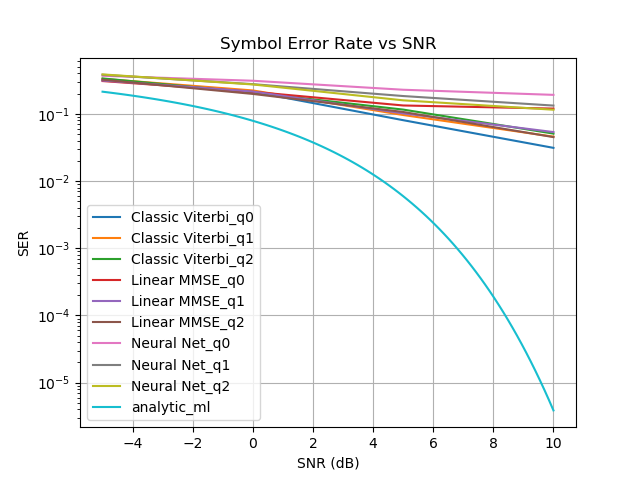
\includegraphics[width=\textwidth,height = 7cm]{results/quant_standard}


\item $P(y_{\mathrm{i}})$
: The randomness of the channel. As each received signal represents a state of the system to which noise may be added. A representative mixture-model can be estimated using a set of received signal training data. 
%Picture of MM
%	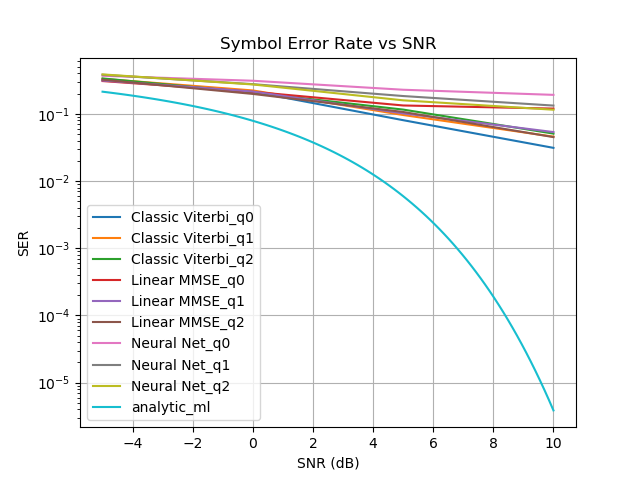
\includegraphics[width=\textwidth,height = 7cm]{results/quant_standard}


\item $P(x_{\mathrm{1 ... L}})$
: Assuming the transmitted symbols are equiprobable, this term can be neglected as all states $x_{\mathrm{1 ... L}}$ will have equal probability. 

\end{itemize}




\section{Simulation Results}
\subsection{System Model}
Consider the received signal 
\begin{equation}
y[k] = \sum_{\mathrm{l=1}}^{\mathrm{L}} a[l]x[k-l] + n[k], \; n[k]  \sim \mathcal{N}(0,1)
\end{equation}

<<<<<<< HEAD
with $x[k-l] \in \{ -1, +1\}$ and $n[k]  \sim \mathcal{N}(0,1)$.  
The resulting signal to noise ratio (SNR) is 
$\frac{E\{x[k]\}}{\sigma^2}$.

Unless noted, the neural network architecture and training are characterized by:
\begin{itemize}
\item Architecture: 4 layers {1, 100, 50, $M^L$}
\item Training Data Examples: 5000
\item Dropout Rate: .5
\item Neural Network Updates: Adam with step size $10^{-3}$ \cite{kingma2014adam}
\item Batch Size: 30 
\item Backpropogation Updates (Epochs): 300
\item Loss Function: Cross Entropy
\end{itemize}


\begin{figure}[H]
	  \caption{Simulation Channels: LTI Channel}
	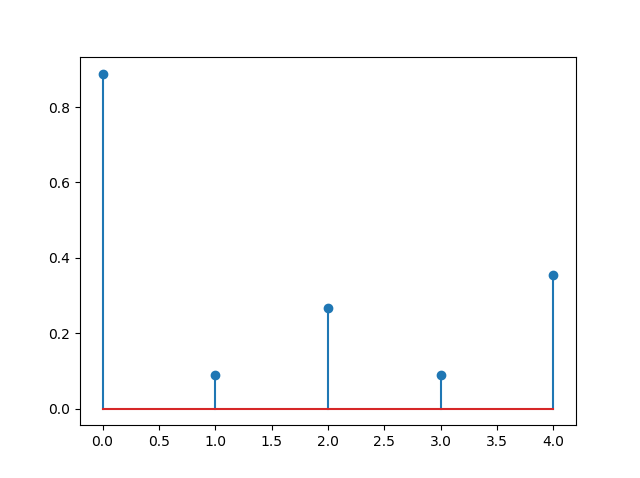
\includegraphics[width=10cm,height = 10cm]{system_model/lti_channel}
	  \label{fig:LTI Channel}
\end{figure}
\begin{figure}[H]
	  \caption{Simulation Channels: Quantizer}
	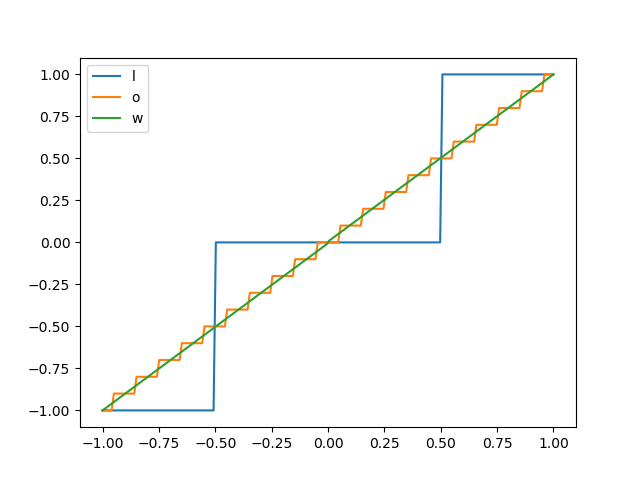
\includegraphics[width=10cm,height = 10cm]{system_model/quantizer}
	  \label{fig:Quantized Channel}
\end{figure}



Adding quantization at matched filter (prior to noise being added)


Details of NN architecture and training

Details of Mixture Model training

\subsection{Results}
Proposed Figures
\begin{figure}[H]
	  \caption{LTI Channel }
	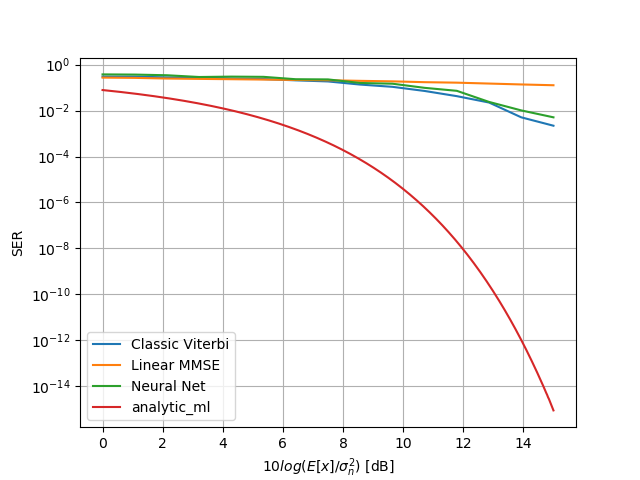
\includegraphics[width=\textwidth,height = 10cm]{results/lti_normal}
	  \label{fig:LTI Channel}
\end{figure}

\begin{figure}[H]
	  \caption{LTI + Quantized Channel }
	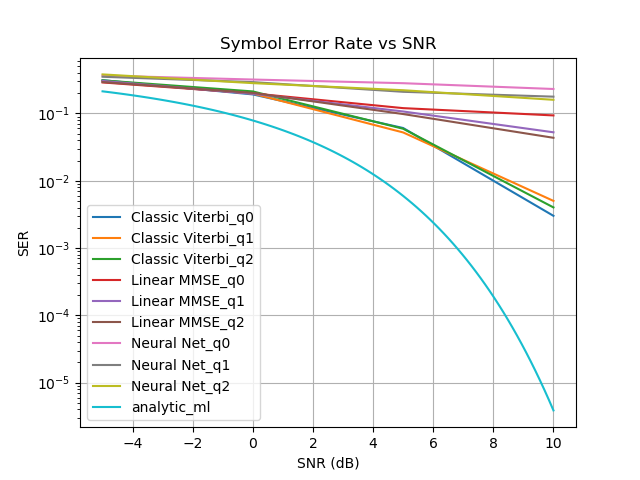
\includegraphics[width=\textwidth,height = 10cm]{results/lti_quantized}
	  \label{fig:LTI_quant Channel}
\end{figure}

\begin{figure}[H]
	  \caption{Reduced State (32 $\rightarrow$ 4) ViterbiNet: LTI Channel}
	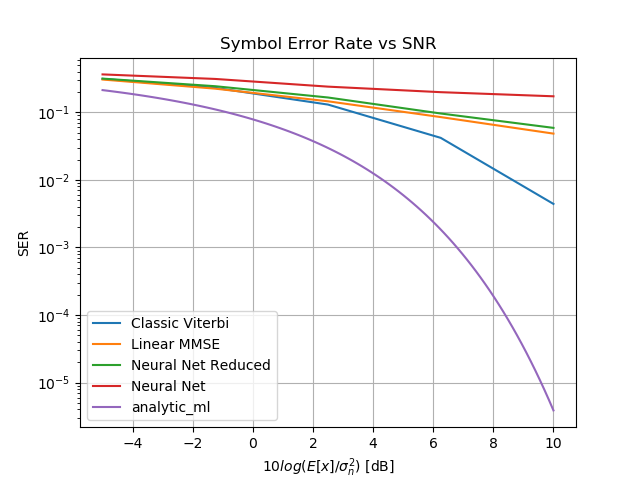
\includegraphics[width=\textwidth,height = 10cm]{results/lti_reduced}
	  \label{fig:reduced_lti}
\end{figure}

\begin{figure}[H]
	  \caption{Reduced State (32 $\rightarrow$ 4) ViterbiNet: LTI + Quantized Channel}
	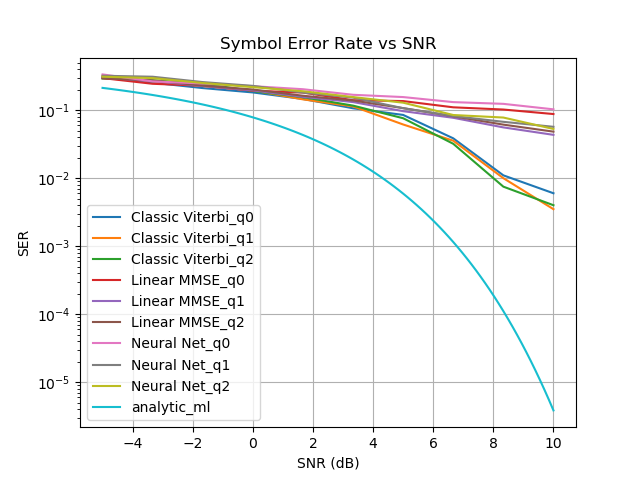
\includegraphics[width=\textwidth,height = 10cm]{results/quantized_reduced}
	  \label{fig:reduced_lti_quantized}
\end{figure}


\subsection*{ViterbiNet}
\subsection*{Reduced State ViterbiNet}
\section{Conclusion}
\subsection{Future Work}
Discuss forward backward (APP) algorithms that could be implemented.

\newpage
\bibliography{mc_report}
\end{document}\documentclass[12pt,a4paper]{report}
\usepackage[utf8]{inputenc}
\usepackage{amsmath}
\usepackage{amsfonts}
\usepackage{amssymb}
\usepackage{graphicx}
\usepackage{float}

\input defs.tex
\bibliographystyle{alpha}
\graphicspath{ {./figures/} }



\title{Neural Network Based Decoding over Molecular Communication Channels}
\author{Peter Hartig}

\begin{document}
\maketitle

\begin{abstract}

\end{abstract}

\newpage
\tableofcontents
\newpage
\section{Notation}
The following notation conventions are used 
Expectation
Conditional Probability 
Argmax
Vector Indexing

\section{Introduction}
Characterizing and obtaining information about communication channels is a fundamental barrier to communication. While optimal and sub-optimal strategies for overcoming this barrier in many contexts have enabled vast and effective communication infrastructure, this barrier still limits communication in others. Molecular Communication channels pose a particularly difficult context in which to overcome this barrier as channel characteristics are often non-linear and may be dependent on the specific transmitted information.
In communication contexts, such as wireless, "Pilot" symbol-streams are often used to mitigate the difficultly in obtaining channel information by provide real-time information supporting an underlying channel model. The low symbol rate of Molecular Communication channels often makes such strategies impractical. However, the success of this data-driven technique in wireless channels suggest that perhaps an alternative, data-driven method may be viable in the Molecular Communication context. One potential data-driven method for characterizing these channels is a neural network. Neural networks have shown to be an effective tool in data-driven approximating of probability distributions.
\par

The general communication channel is equivalent to a conditional probability $P(x|y)$, in which $x$ is transmitted information and $y$ is received information.  $P(x|y)$ takes into account the (potentially random) channel through which the information $x$ passes, and random noise added prior to receiving $y$. The communication problem entails optimizing a form of $P(x|y)$ over a set of possible, transmitted information $x$. In general, sub-optimal solutions do not require perfect knowledge of the distribution $P(x|y)$ and may be used when $P(x|y)$ is unknown or impractical to obtain. In this work, a neural network is used to estimate $P(x|y)$.

\section{Background}

\subsection{MLSE}
The form of $P(x|y)$ used for detection in this work is
$\underset{x}{\text{argmin}} \; P(y|x) $ . This optimization, known as Maximum Likelihood Sequence Estimation (MLSE), over the set of all possible $x$ is exponentially complex in the cardinaltiy of $x$ . Information about the communication channel can, however, reduce the complexity of this problem. In order to illustrate this reduction, the following example is proposed.
\par
Consider the communication channel over which a causal, linear, and time invariant combination of a set of the transmitted information is received. 

\begin{equation}
y[k] = \sum_{\mathrm{l=1}}^{\mathrm{L}} a[l]x[k-l]
\end{equation}

In this case, $P(y|x)$ can be rewritten as
$\prod P(y_{\mathrm{i}}|x_{\mathrm{i-L+1}}^{\mathrm{i}}) = \sum
log(P(y_{\mathrm{i}}|x_{\mathrm{i-L+1}}^{\mathrm{i}}) )$.
The sequence of received symbols $\mathbf{y}$ can be equivalently represented the by trellis:

TODO IMPORT Trellis picture
in which each time-point k represents a unique set of L transmitted symbols 
$x[k-l]$ $ \forall l \in {1..L}$. Due to the finite number of states that channel can be in at a given time, MLSE can be performed using the Viterbi Algorithm over this trellis. 

Viterbi Algorithm:

    \noindent\rule[10pt]{\textwidth}{0.4pt}
    {\footnotesize
    \begin{tabbing}
        {\bf given} $P(y_{\mathrm{i}}|x_{\mathrm{i-L+1}}^{\mathrm{i}}) \; \forall i \in {1..N}$ . \\*[\smallskipamount]
        Let $\lambda := \lambda^{k-1}$. \\*[\smallskipamount]
        {\bf for $i = 1..N $} \\
         \qquad \= {\bf for each state $s$ at time $i$}\\
        \qquad \qquad \= 1.\ Let $\mathrm{Path}_{s} := \prox_{\lambda g}(x^{k} - \lambda \nabla f(x^{k}))$. \\
        \> 2.\ {\bf break if} $f(z) \leq \hat{f}_{\lambda}(z, x^{k})$. \\
        \> 3.\ Update $\lambda := \beta \lambda$. \\*[\smallskipamount]
        {\bf return} $\underset{s}{\text{argmin}} \; cost[i] $, $x^{k+1}:=z$.
    \end{tabbing}}
    \noindent\rule[10pt]{\textwidth}{0.4pt}


For finite state, causal channels, MLSE reduces to the Viterbi Algorithm. Note that while Viterbi algorithm does have exponential complexity in the length of the channle (i.e. L), complexity is linear in the length of the sequence. 


\subsection{ViterbiNet}
As suggested in the introduction, despite the reduction in complexity offered by the Viterbi Algorithm for MLSE, the individual metrics used each step of the algorithm 
$P(y_{\mathrm{i}}|x_{\mathrm{i-L+1}}^{\mathrm{i}}) $ require knowledge of the channel which may be difficult to obtain. To estimate this distribution using a neural network, Baye's Rule is used. 
\begin{equation}
P(y_{\mathrm{i}}|x_{\mathrm{1 ... L}}) = 
\frac
{P(x_{\mathrm{1 ... L}}|y_{\mathrm{i}})P(y_{\mathrm{i}})}
{P(x_{\mathrm{1 ... L}})}
\end{equation}

These terms can be interpreted as:

\begin{itemize}
\item $P(x_{\mathrm{1 ... L}}|y_{\mathrm{i}})$
: The probability of being in a channel state given the corresponding received symbol from that time point. In the case of a finite number of states, such a probability can be estimated using a neural network for classification of received signals into channel states. 
%Picture of NN
%	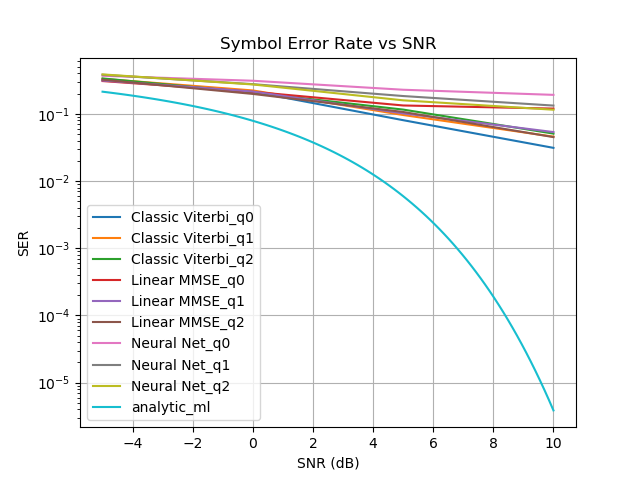
\includegraphics[width=\textwidth,height = 7cm]{results/quant_standard}


\item $P(y_{\mathrm{i}})$
: The randomness of the channel. As each received signal represents a state of the system to which noise may be added. A representative mixture-model can be estimated using a set of received signal training data. 
%Picture of MM
%	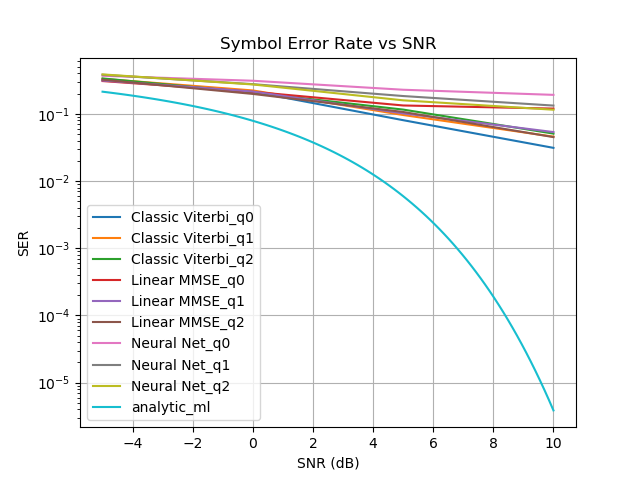
\includegraphics[width=\textwidth,height = 7cm]{results/quant_standard}


\item $P(x_{\mathrm{1 ... L}})$
: Assuming the transmitted symbols are equiprobable, this term can be neglected as all states $x_{\mathrm{1 ... L}}$ will have equal probability. 

\end{itemize}




\section{Simulation Results}
\subsection{System Model}
Consider the received signal 
\begin{equation}
y[k] = \sum_{\mathrm{l=1}}^{\mathrm{L}} a[l]x[k-l] + n[k], \; n[k]  \sim \mathcal{N}(0,1)
\end{equation}

with $x[k-l] \in \{ -1, +1\}$ and $n[k]  \sim \mathcal{N}(0,1)$.  
The resulting signal to noise ratio (SNR) is 
$\frac{E\{x[k]\}}{\sigma^2}$.

Unless noted, the neural network architecture and training are characterized by:
\begin{itemize}
\item Architecture: 4 layers {1, 100, 50, $M^L$}
\item Training Data Examples: 5000
\item Dropout Rate: .5
\item Neural Network Updates: Adam with step size $10^{-3}$ \cite{kingma2014adam}
\item Batch Size: 30 
\item Backpropogation Updates (Epochs): 300
\item Loss Function: Cross Entropy
\end{itemize}


\begin{figure}[H]
	  \caption{Simulation Channels: LTI Channel}
	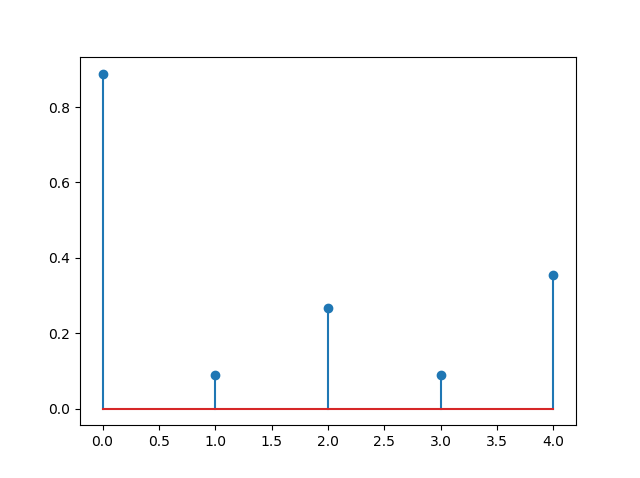
\includegraphics[width=10cm,height = 10cm]{system_model/lti_channel}
	  \label{fig:LTI Channel}
\end{figure}
\begin{figure}[H]
	  \caption{Simulation Channels: Quantizer}
	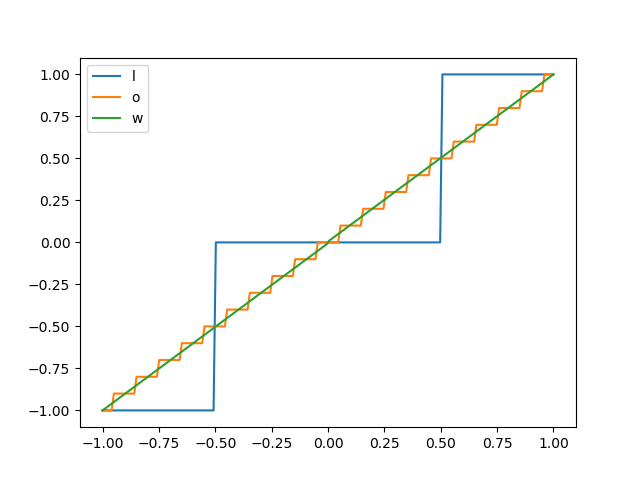
\includegraphics[width=10cm,height = 10cm]{system_model/quantizer}
	  \label{fig:Quantized Channel}
\end{figure}



Adding quantization at matched filter (prior to noise being added)


Details of NN architecture and training

Details of Mixture Model training

\subsection{Results}
Proposed Figures
\begin{figure}[H]
	  \caption{LTI Channel }
	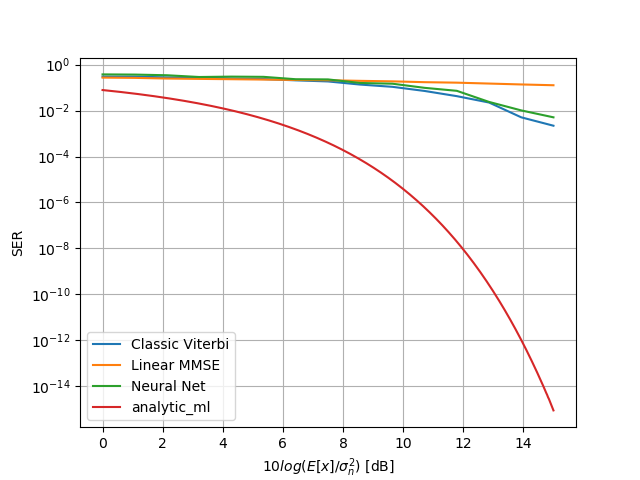
\includegraphics[width=\textwidth,height = 10cm]{results/lti_normal}
	  \label{fig:LTI Channel}
\end{figure}

\begin{figure}[H]
	  \caption{LTI + Quantized Channel }
	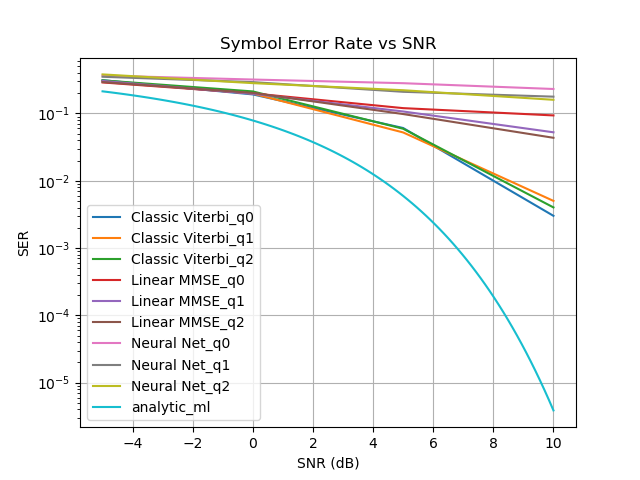
\includegraphics[width=\textwidth,height = 10cm]{results/lti_quantized}
	  \label{fig:LTI_quant Channel}
\end{figure}

\begin{figure}[H]
	  \caption{Reduced State (32 $\rightarrow$ 4) ViterbiNet: LTI Channel}
	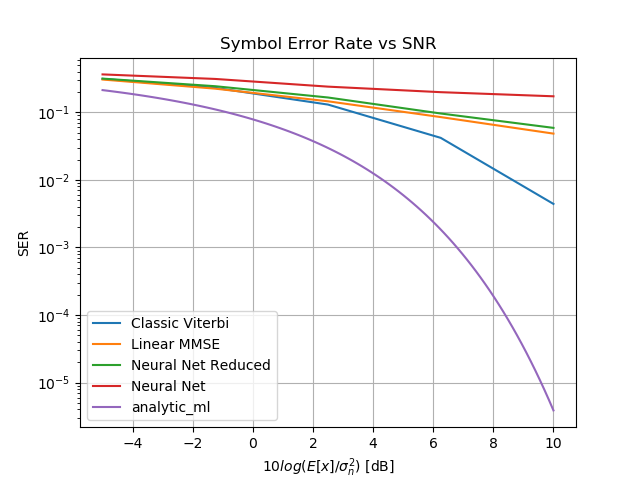
\includegraphics[width=\textwidth,height = 10cm]{results/lti_reduced}
	  \label{fig:reduced_lti}
\end{figure}

\begin{figure}[H]
	  \caption{Reduced State (32 $\rightarrow$ 4) ViterbiNet: LTI + Quantized Channel}
	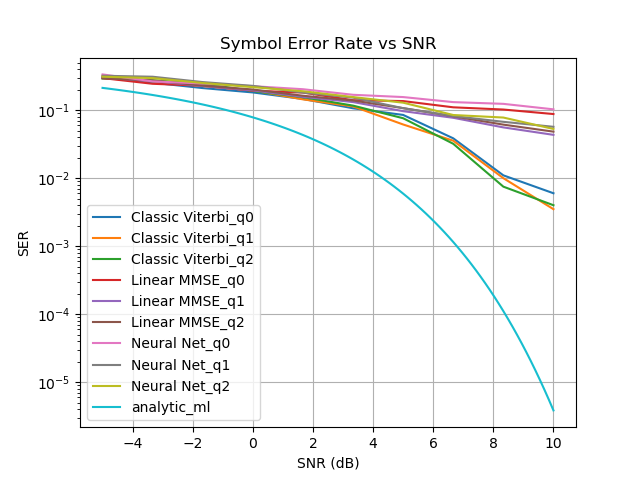
\includegraphics[width=\textwidth,height = 10cm]{results/quantized_reduced}
	  \label{fig:reduced_lti_quantized}
\end{figure}


\subsection*{ViterbiNet}
\subsection*{Reduced State ViterbiNet}
\section{Conclusion}
\subsection{Future Work}
Discuss forward backward (APP) algorithms that could be implemented.

\newpage
\bibliography{mc_report}
\end{document}\documentclass[12pt,a4paper]{report}
\usepackage[utf8]{inputenc}
\usepackage{amsmath}
\usepackage{amsfonts}
\usepackage{amssymb}
\usepackage{graphicx}
\usepackage{float}

\input defs.tex
\bibliographystyle{alpha}
\graphicspath{ {./figures/} }



\title{Neural Network Based Decoding over Molecular Communication Channels}
\author{Peter Hartig}

\begin{document}
\maketitle

\begin{abstract}

\end{abstract}

\newpage
\tableofcontents
\newpage
\section{Notation}
The following notation conventions are used 
Expectation
Conditional Probability 
Argmax
Vector Indexing

\section{Introduction}
Characterizing and obtaining information about communication channels is a fundamental barrier to communication. While optimal and sub-optimal strategies for overcoming this barrier in many contexts have enabled vast and effective communication infrastructure, this barrier still limits communication in others. Molecular Communication channels pose a particularly difficult context in which to overcome this barrier as channel characteristics are often non-linear and may be dependent on the specific transmitted information.
In communication contexts, such as wireless, "Pilot" symbol-streams are often used to mitigate the difficultly in obtaining channel information by provide real-time information supporting an underlying channel model. The low symbol rate of Molecular Communication channels often makes such strategies impractical. However, the success of this data-driven technique in wireless channels suggest that perhaps an alternative, data-driven method may be viable in the Molecular Communication context. One potential data-driven method for characterizing these channels is a neural network. Neural networks have shown to be an effective tool in data-driven approximating of probability distributions.
\par

The general communication channel is equivalent to a conditional probability $P(x|y)$, in which $x$ is transmitted information and $y$ is received information.  $P(x|y)$ takes into account the (potentially random) channel through which the information $x$ passes, and random noise added prior to receiving $y$. The communication problem entails optimizing a form of $P(x|y)$ over a set of possible, transmitted information $x$. In general, sub-optimal solutions do not require perfect knowledge of the distribution $P(x|y)$ and may be used when $P(x|y)$ is unknown or impractical to obtain. In this work, a neural network is used to estimate $P(x|y)$.

\section{Background}

\subsection{MLSE}
The form of $P(x|y)$ used for detection in this work is
$\underset{x}{\text{argmin}} \; P(y|x) $ . This optimization, known as Maximum Likelihood Sequence Estimation (MLSE), over the set of all possible $x$ is exponentially complex in the cardinaltiy of $x$ . Information about the communication channel can, however, reduce the complexity of this problem. In order to illustrate this reduction, the following example is proposed.
\par
Consider the communication channel over which a causal, linear, and time invariant combination of a set of the transmitted information is received. 

\begin{equation}
y[k] = \sum_{\mathrm{l=1}}^{\mathrm{L}} a[l]x[k-l]
\end{equation}

In this case, $P(y|x)$ can be rewritten as
$\prod P(y_{\mathrm{i}}|x_{\mathrm{i-L+1}}^{\mathrm{i}}) = \sum
log(P(y_{\mathrm{i}}|x_{\mathrm{i-L+1}}^{\mathrm{i}}) )$.
The sequence of received symbols $\mathbf{y}$ can be equivalently represented the by trellis:

TODO IMPORT Trellis picture
in which each time-point k represents a unique set of L transmitted symbols 
$x[k-l]$ $ \forall l \in {1..L}$. Due to the finite number of states that channel can be in at a given time, MLSE can be performed using the Viterbi Algorithm over this trellis. 

Viterbi Algorithm:

    \noindent\rule[10pt]{\textwidth}{0.4pt}
    {\footnotesize
    \begin{tabbing}
        {\bf given} $P(y_{\mathrm{i}}|x_{\mathrm{i-L+1}}^{\mathrm{i}}) \; \forall i \in {1..N}$ . \\*[\smallskipamount]
        Let $\lambda := \lambda^{k-1}$. \\*[\smallskipamount]
        {\bf for $i = 1..N $} \\
         \qquad \= {\bf for each state $s$ at time $i$}\\
        \qquad \qquad \= 1.\ Let $\mathrm{Path}_{s} := \prox_{\lambda g}(x^{k} - \lambda \nabla f(x^{k}))$. \\
        \> 2.\ {\bf break if} $f(z) \leq \hat{f}_{\lambda}(z, x^{k})$. \\
        \> 3.\ Update $\lambda := \beta \lambda$. \\*[\smallskipamount]
        {\bf return} $\underset{s}{\text{argmin}} \; cost[i] $, $x^{k+1}:=z$.
    \end{tabbing}}
    \noindent\rule[10pt]{\textwidth}{0.4pt}

=======
with $x[k-l] \in \{ -1, +1\}$ and $n[k]  \sim \mathcal{N}(0,1)$
with signal to noise ratio (SNR) 
$\frac{E\{x[k]\}}{\sigma^2}$
>>>>>>> parent of b93eac3... some changes to report

For finite state, causal channels, MLSE reduces to the Viterbi Algorithm. Note that while Viterbi algorithm does have exponential complexity in the length of the channle (i.e. L), complexity is linear in the length of the sequence. 


\subsection{ViterbiNet}
As suggested in the introduction, despite the reduction in complexity offered by the Viterbi Algorithm for MLSE, the individual metrics used each step of the algorithm 
$P(y_{\mathrm{i}}|x_{\mathrm{i-L+1}}^{\mathrm{i}}) $ require knowledge of the channel which may be difficult to obtain. To estimate this distribution using a neural network, Baye's Rule is used. 
\begin{equation}
P(y_{\mathrm{i}}|x_{\mathrm{1 ... L}}) = 
\frac
{P(x_{\mathrm{1 ... L}}|y_{\mathrm{i}})P(y_{\mathrm{i}})}
{P(x_{\mathrm{1 ... L}})}
\end{equation}

These terms can be interpreted as:

\begin{itemize}
\item $P(x_{\mathrm{1 ... L}}|y_{\mathrm{i}})$
: The probability of being in a channel state given the corresponding received symbol from that time point. In the case of a finite number of states, such a probability can be estimated using a neural network for classification of received signals into channel states. 
%Picture of NN
%	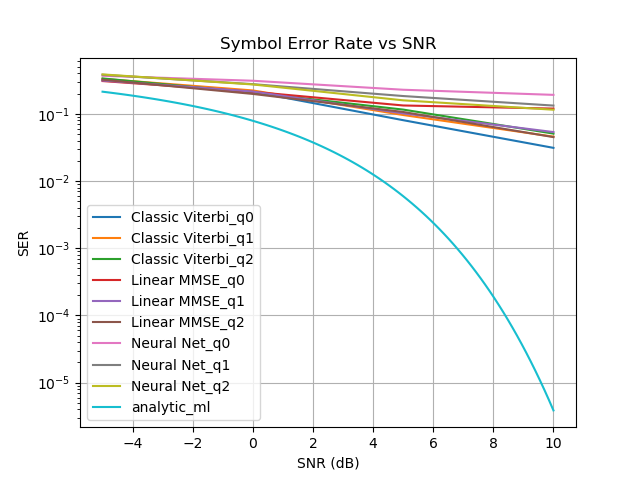
\includegraphics[width=\textwidth,height = 7cm]{results/quant_standard}


\item $P(y_{\mathrm{i}})$
: The randomness of the channel. As each received signal represents a state of the system to which noise may be added. A representative mixture-model can be estimated using a set of received signal training data. 
%Picture of MM
%	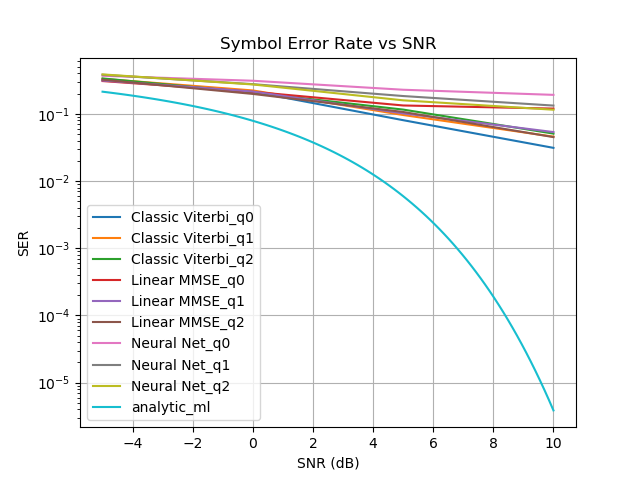
\includegraphics[width=\textwidth,height = 7cm]{results/quant_standard}


\item $P(x_{\mathrm{1 ... L}})$
: Assuming the transmitted symbols are equiprobable, this term can be neglected as all states $x_{\mathrm{1 ... L}}$ will have equal probability. 

\end{itemize}




\section{Simulation Results}
\subsection{System Model}
Consider the received signal 
\begin{equation}
y[k] = \sum_{\mathrm{l=1}}^{\mathrm{L}} a[l]x[k-l] + n[k], \; n[k]  \sim \mathcal{N}(0,1)
\end{equation}

with $x[k-l] \in \{ -1, +1\}$ and $n[k]  \sim \mathcal{N}(0,1)$.  
The resulting signal to noise ratio (SNR) is 
$\frac{E\{x[k]\}}{\sigma^2}$.

Unless noted, the neural network architecture and training are characterized by:
\begin{itemize}
\item Architecture: 4 layers {1, 100, 50, $M^L$}
\item Training Data Examples: 5000
\item Dropout Rate: .5
\item Neural Network Updates: Adam with step size $10^{-3}$ \cite{kingma2014adam}
\item Batch Size: 30 
\item Backpropogation Updates (Epochs): 300
\item Loss Function: Cross Entropy
\end{itemize}


\begin{figure}[H]
	  \caption{Simulation Channels: LTI Channel}
	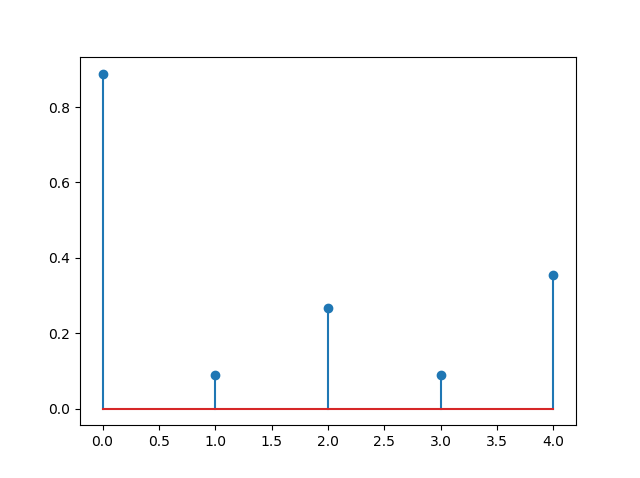
\includegraphics[width=10cm,height = 10cm]{system_model/lti_channel}
	  \label{fig:LTI Channel}
\end{figure}
\begin{figure}[H]
	  \caption{Simulation Channels: Quantizer}
	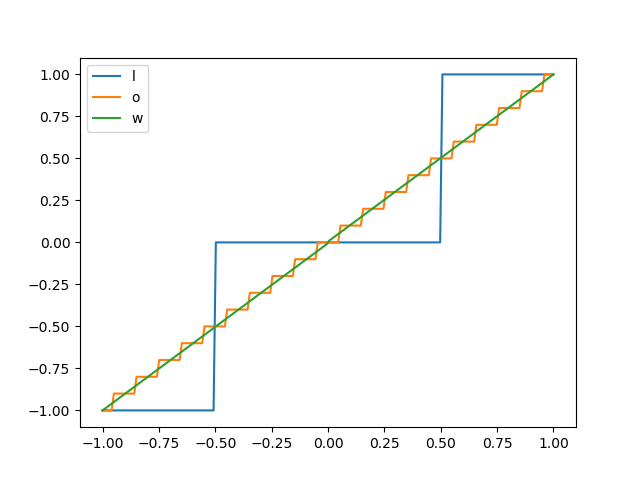
\includegraphics[width=10cm,height = 10cm]{system_model/quantizer}
	  \label{fig:Quantized Channel}
\end{figure}



Adding quantization at matched filter (prior to noise being added)


Details of NN architecture and training

Details of Mixture Model training

\subsection{Results}
Proposed Figures
\begin{figure}[H]
	  \caption{LTI Channel }
	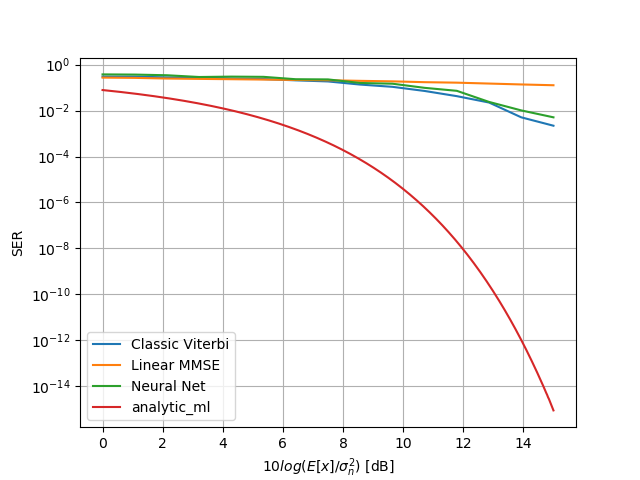
\includegraphics[width=\textwidth,height = 10cm]{results/lti_normal}
	  \label{fig:LTI Channel}
\end{figure}

\begin{figure}[H]
	  \caption{LTI + Quantized Channel }
	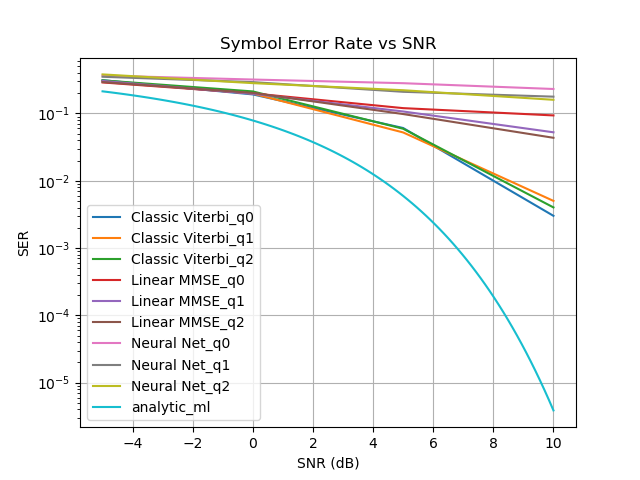
\includegraphics[width=\textwidth,height = 10cm]{results/lti_quantized}
	  \label{fig:LTI_quant Channel}
\end{figure}

\begin{figure}[H]
	  \caption{Reduced State (32 $\rightarrow$ 4) ViterbiNet: LTI Channel}
	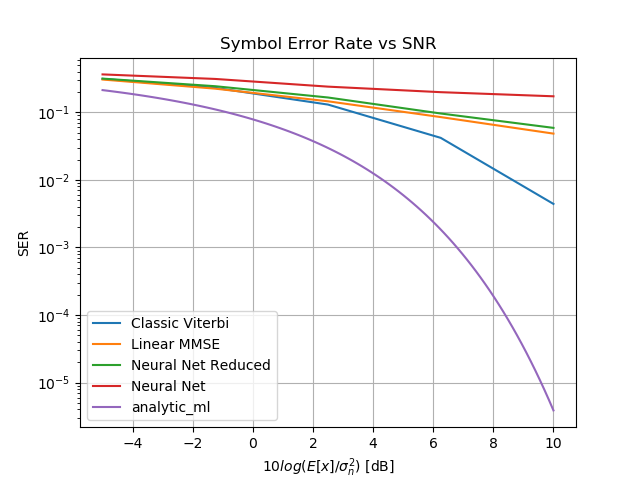
\includegraphics[width=\textwidth,height = 10cm]{results/lti_reduced}
	  \label{fig:reduced_lti}
\end{figure}

\begin{figure}[H]
	  \caption{Reduced State (32 $\rightarrow$ 4) ViterbiNet: LTI + Quantized Channel}
	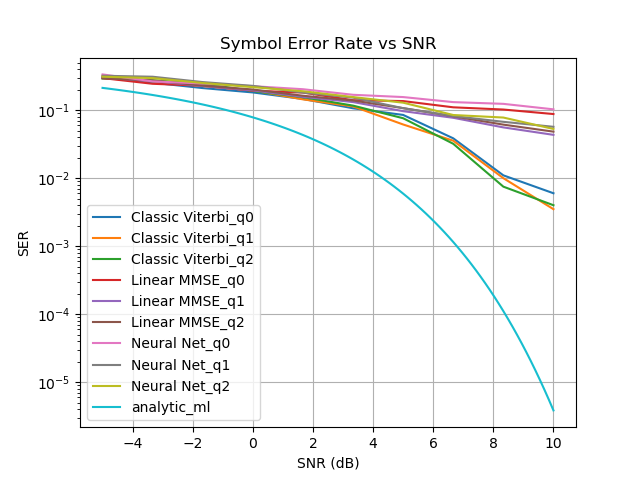
\includegraphics[width=\textwidth,height = 10cm]{results/quantized_reduced}
	  \label{fig:reduced_lti_quantized}
\end{figure}


\subsection*{ViterbiNet}
\subsection*{Reduced State ViterbiNet}
\section{Conclusion}
\subsection{Future Work}
Discuss forward backward (APP) algorithms that could be implemented.

\newpage
\bibliography{mc_report}
\end{document}\documentclass[12pt,a4paper]{report}
\usepackage[utf8]{inputenc}
\usepackage{amsmath}
\usepackage{amsfonts}
\usepackage{amssymb}
\usepackage{graphicx}
\usepackage{float}

\input defs.tex
\bibliographystyle{alpha}
\graphicspath{ {./figures/} }



\title{Neural Network Based Decoding over Molecular Communication Channels}
\author{Peter Hartig}

\begin{document}
\maketitle

\begin{abstract}

\end{abstract}

\newpage
\tableofcontents
\newpage
\section{Notation}
The following notation conventions are used 
Expectation
Conditional Probability 
Argmax
Vector Indexing

\section{Introduction}
Characterizing and obtaining information about communication channels is a fundamental barrier to communication. While optimal and sub-optimal strategies for overcoming this barrier in many contexts have enabled vast and effective communication infrastructure, this barrier still limits communication in others. Molecular Communication channels pose a particularly difficult context in which to overcome this barrier as channel characteristics are often non-linear and may be dependent on the specific transmitted information.
In communication contexts, such as wireless, "Pilot" symbol-streams are often used to mitigate the difficultly in obtaining channel information by provide real-time information supporting an underlying channel model. The low symbol rate of Molecular Communication channels often makes such strategies impractical. However, the success of this data-driven technique in wireless channels suggest that perhaps an alternative, data-driven method may be viable in the Molecular Communication context. One potential data-driven method for characterizing these channels is a neural network. Neural networks have shown to be an effective tool in data-driven approximating of probability distributions.
\par

The general communication channel is equivalent to a conditional probability $P(x|y)$, in which $x$ is transmitted information and $y$ is received information.  $P(x|y)$ takes into account the (potentially random) channel through which the information $x$ passes, and random noise added prior to receiving $y$. The communication problem entails optimizing a form of $P(x|y)$ over a set of possible, transmitted information $x$. In general, sub-optimal solutions do not require perfect knowledge of the distribution $P(x|y)$ and may be used when $P(x|y)$ is unknown or impractical to obtain. In this work, a neural network is used to estimate $P(x|y)$.

\section{Background}

\subsection{MLSE}
The form of $P(x|y)$ used for detection in this work is
$\underset{x}{\text{argmin}} \; P(y|x) $ . This optimization, known as Maximum Likelihood Sequence Estimation (MLSE), over the set of all possible $x$ is exponentially complex in the cardinaltiy of $x$ . Information about the communication channel can, however, reduce the complexity of this problem. In order to illustrate this reduction, the following example is proposed.
\par
Consider the communication channel over which a causal, linear, and time invariant combination of a set of the transmitted information is received. 

\begin{equation}
y[k] = \sum_{\mathrm{l=1}}^{\mathrm{L}} a[l]x[k-l]
\end{equation}

In this case, $P(y|x)$ can be rewritten as
$\prod P(y_{\mathrm{i}}|x_{\mathrm{i-L+1}}^{\mathrm{i}}) = \sum
log(P(y_{\mathrm{i}}|x_{\mathrm{i-L+1}}^{\mathrm{i}}) )$.
The sequence of received symbols $\mathbf{y}$ can be equivalently represented the by trellis:

TODO IMPORT Trellis picture
in which each time-point k represents a unique set of L transmitted symbols 
$x[k-l]$ $ \forall l \in {1..L}$. Due to the finite number of states that channel can be in at a given time, MLSE can be performed using the Viterbi Algorithm over this trellis. 

Viterbi Algorithm:

    \noindent\rule[10pt]{\textwidth}{0.4pt}
    {\footnotesize
    \begin{tabbing}
        {\bf given} $P(y_{\mathrm{i}}|x_{\mathrm{i-L+1}}^{\mathrm{i}}) \; \forall i \in {1..N}$ . \\*[\smallskipamount]
        Let $\lambda := \lambda^{k-1}$. \\*[\smallskipamount]
        {\bf for $i = 1..N $} \\
         \qquad \= {\bf for each state $s$ at time $i$}\\
        \qquad \qquad \= 1.\ Let $\mathrm{Path}_{s} := \prox_{\lambda g}(x^{k} - \lambda \nabla f(x^{k}))$. \\
        \> 2.\ {\bf break if} $f(z) \leq \hat{f}_{\lambda}(z, x^{k})$. \\
        \> 3.\ Update $\lambda := \beta \lambda$. \\*[\smallskipamount]
        {\bf return} $\underset{s}{\text{argmin}} \; cost[i] $, $x^{k+1}:=z$.
    \end{tabbing}}
    \noindent\rule[10pt]{\textwidth}{0.4pt}


For finite state, causal channels, MLSE reduces to the Viterbi Algorithm. Note that while Viterbi algorithm does have exponential complexity in the length of the channle (i.e. L), complexity is linear in the length of the sequence. 


\subsection{ViterbiNet}
As suggested in the introduction, despite the reduction in complexity offered by the Viterbi Algorithm for MLSE, the individual metrics used each step of the algorithm 
$P(y_{\mathrm{i}}|x_{\mathrm{i-L+1}}^{\mathrm{i}}) $ require knowledge of the channel which may be difficult to obtain. To estimate this distribution using a neural network, Baye's Rule is used. 
\begin{equation}
P(y_{\mathrm{i}}|x_{\mathrm{1 ... L}}) = 
\frac
{P(x_{\mathrm{1 ... L}}|y_{\mathrm{i}})P(y_{\mathrm{i}})}
{P(x_{\mathrm{1 ... L}})}
\end{equation}

These terms can be interpreted as:

\begin{itemize}
\item $P(x_{\mathrm{1 ... L}}|y_{\mathrm{i}})$
: The probability of being in a channel state given the corresponding received symbol from that time point. In the case of a finite number of states, such a probability can be estimated using a neural network for classification of received signals into channel states. 
%Picture of NN
%	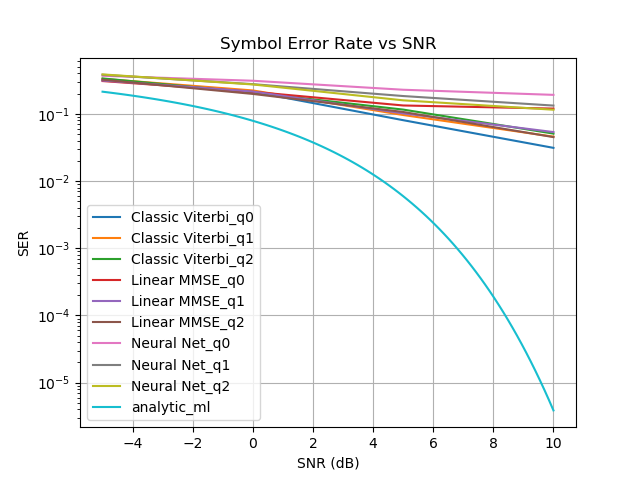
\includegraphics[width=\textwidth,height = 7cm]{results/quant_standard}


\item $P(y_{\mathrm{i}})$
: The randomness of the channel. As each received signal represents a state of the system to which noise may be added. A representative mixture-model can be estimated using a set of received signal training data. 
%Picture of MM
%	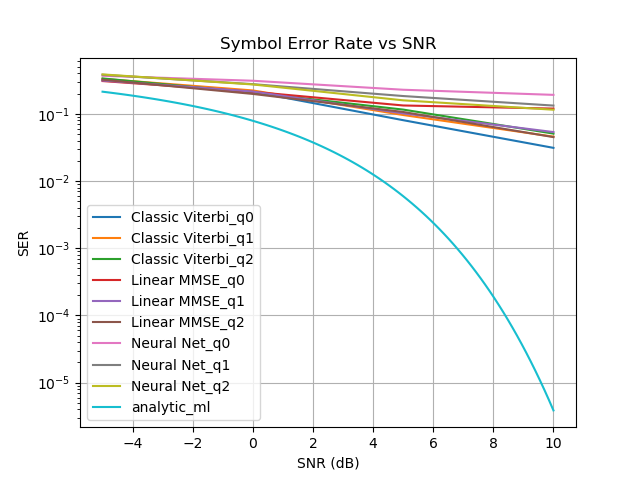
\includegraphics[width=\textwidth,height = 7cm]{results/quant_standard}


\item $P(x_{\mathrm{1 ... L}})$
: Assuming the transmitted symbols are equiprobable, this term can be neglected as all states $x_{\mathrm{1 ... L}}$ will have equal probability. 

\end{itemize}




\section{Simulation Results}
\subsection{System Model}
Consider the received signal 
\begin{equation}
y[k] = \sum_{\mathrm{l=1}}^{\mathrm{L}} a[l]x[k-l] + n[k], \; n[k]  \sim \mathcal{N}(0,1)
\end{equation}

with $x[k-l] \in \{ -1, +1\}$ and $n[k]  \sim \mathcal{N}(0,1)$.  
The resulting signal to noise ratio (SNR) is 
$\frac{E\{x[k]\}}{\sigma^2}$.

Unless noted, the neural network architecture and training are characterized by:
\begin{itemize}
\item Architecture: 4 layers {1, 100, 50, $M^L$}
\item Training Data Examples: 5000
\item Dropout Rate: .5
\item Neural Network Updates: Adam with step size $10^{-3}$ \cite{kingma2014adam}
\item Batch Size: 30 
\item Backpropogation Updates (Epochs): 300
\item Loss Function: Cross Entropy
\end{itemize}


\begin{figure}[H]
	  \caption{Simulation Channels: LTI Channel}
	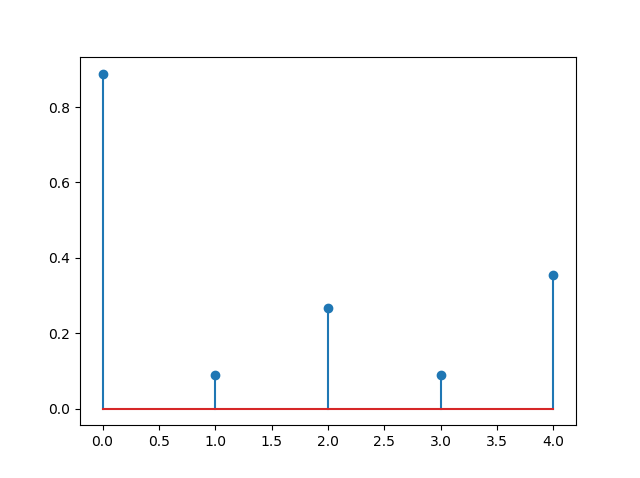
\includegraphics[width=10cm,height = 10cm]{system_model/lti_channel}
	  \label{fig:LTI Channel}
\end{figure}
\begin{figure}[H]
	  \caption{Simulation Channels: Quantizer}
	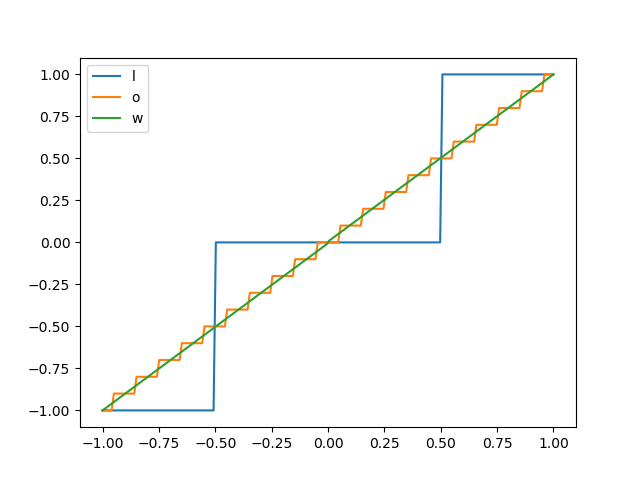
\includegraphics[width=10cm,height = 10cm]{system_model/quantizer}
	  \label{fig:Quantized Channel}
\end{figure}



Adding quantization at matched filter (prior to noise being added)


Details of NN architecture and training

Details of Mixture Model training

\subsection{Results}
Proposed Figures
\begin{figure}[H]
	  \caption{LTI Channel }
	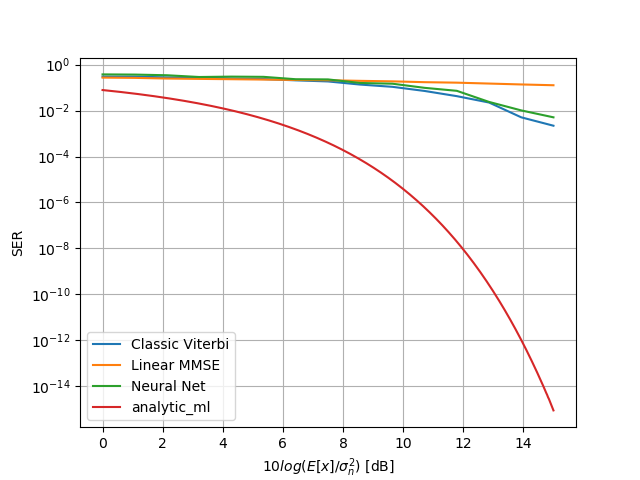
\includegraphics[width=\textwidth,height = 10cm]{results/lti_normal}
	  \label{fig:LTI Channel}
\end{figure}

\begin{figure}[H]
	  \caption{LTI + Quantized Channel }
	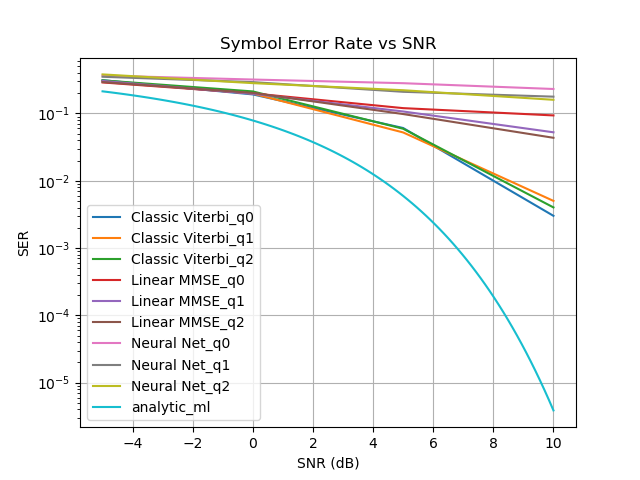
\includegraphics[width=\textwidth,height = 10cm]{results/lti_quantized}
	  \label{fig:LTI_quant Channel}
\end{figure}

\begin{figure}[H]
	  \caption{Reduced State (32 $\rightarrow$ 4) ViterbiNet: LTI Channel}
	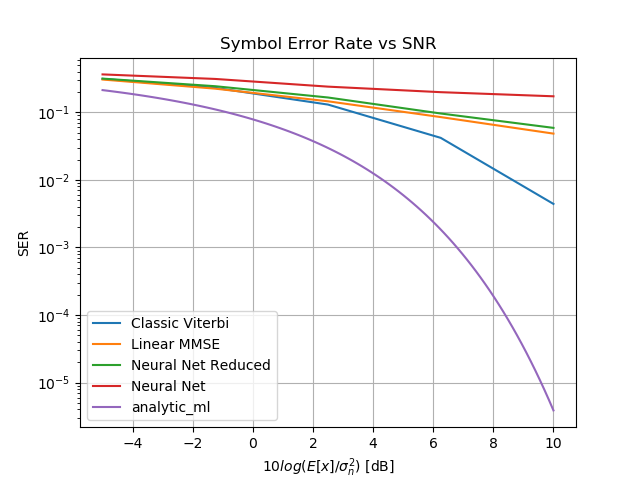
\includegraphics[width=\textwidth,height = 10cm]{results/lti_reduced}
	  \label{fig:reduced_lti}
\end{figure}

\begin{figure}[H]
	  \caption{Reduced State (32 $\rightarrow$ 4) ViterbiNet: LTI + Quantized Channel}
	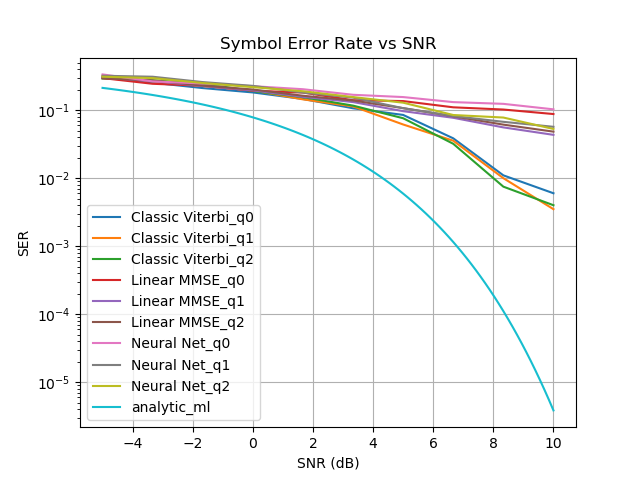
\includegraphics[width=\textwidth,height = 10cm]{results/quantized_reduced}
	  \label{fig:reduced_lti_quantized}
\end{figure}


\subsection*{ViterbiNet}
\subsection*{Reduced State ViterbiNet}
\section{Conclusion}
\subsection{Future Work}
Discuss forward backward (APP) algorithms that could be implemented.

\newpage
\bibliography{mc_report}
\end{document}